\subsection{Algorithm Testing}
Multiple different algorithms have been investigated for this report; standard evolution against n+n evolution, and local sensing against space aware sensing. These two factors combine to provide four statistical comparisons between algorithms:
\begin{enumerate}
  \item \verb|local-standard| vs \verb|local-n+n|
  \item \verb|space_aware-standard| vs \verb|space_aware-n+n|
  \item \verb|local-standard| vs \verb|space_aware-standard|
  \item \verb|local-n+n| vs \verb|space_aware-n+n|
\end{enumerate}
Each algorithm was ran 10 times with a population of 200 for 500 generations, an average of these runs was then computed to provide a fair graphical representation of the performance of each algorithm.

Statistical analysis involved performing a Mann-Whitney-U test at each generation, where a sample consisted of the average value for each run of the algorithm to give a total of 10 samples per generation, per algorithm. A difference of means $m$ was also calculated at each generation. This $p$, $U$, $m$ can then be averaged for all generations to give an average statistic over all generations.

\subsubsection{standard evolution compared to n+n evolution}

Figure \ref{local} compares standard evolution to n+n for local collision sensing, while \verb|local-standard| was the prevailing algorithm after 500 generations, \verb|local-n+n| is consistently performs better from generation 0 until a crossover point at approximately 50 score. Average Mann-Whitney-U and difference of means are:
$$
U = 32.8, p = 0.39137, m = 8.9
$$
As $p > 0.05$, changing evolution selection methods for local sensing is not statistically significant.
\bigskip

Figure \ref{space_aware} compares standard to n+n evolution for space aware collision sensing. As shown in the graph, n+n performed significantly better than standard evolution, though standard deviation was large. Standard evolution struggled to make any progress Throughout generations, with a consistently average score throughout generations of 0. Average Mann-Whitney-U and difference of means are:
$$
U = 0.0, p = 0.00018, m = 6.7
$$
Changing evolution selection methods for space aware sensing is statistically significant as $p < 0.05$. While the difference of means $m$ does not immediately suggest a large effect size, when considering figure \ref{space_aware} the data shows that n+n evolution allows space aware sensing to be a viable collision detection method unlike standard evolution.

\begin{figure}[h]
  \centering
  \begin{minipage}{.5\textwidth}
    \centering
    \captionsetup{width=.8\linewidth}
    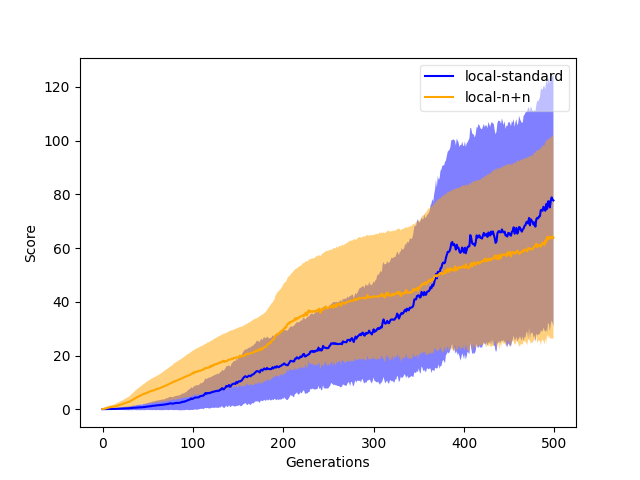
\includegraphics[width=1 \linewidth]{local}
    \caption{\texttt{local-standard} compared to \texttt{local-n+n} over 500 generations}
    \label{local}
  \end{minipage}%
  \begin{minipage}{.5\textwidth}
    \centering
    \captionsetup{width=.8\linewidth}
    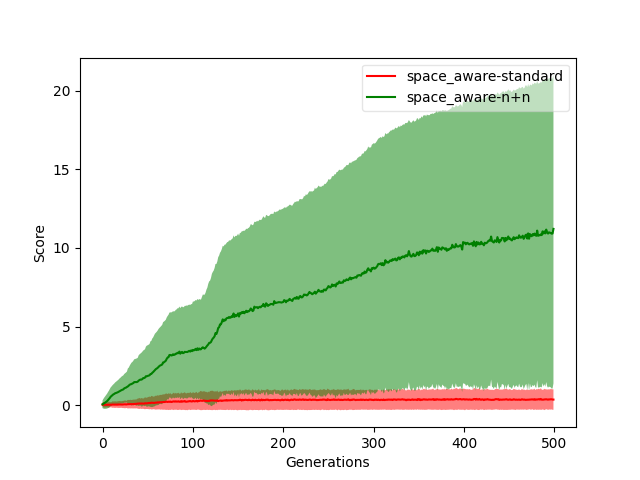
\includegraphics[width=1\linewidth]{space_aware}
    \caption{\texttt{space\_aware-standard} compared to \texttt{space\_aware-n+n} over 500 generations}
    \label{space_aware}
  \end{minipage}
\end{figure}

